\section{Modellierung von Geschäftsprozessen}

\subsection{Grundlagen zur Geschäftsprozessmodellierung}
    \subsubsection*{Eigenschaften von Prozessmodellen}
        Modelle bilden reale oder imaginäre Sachverhalte ab und sind abstrahiert, um relevante Details für den jeweiligen Verwendungszweck zu erfassen.
    \subsubsection*{Verwendungszwecke}
        Organisatorische Anwendungsfälle (Verständnis, Kommunikation, Analyse, Verbesserung, Weiterentwicklung) und Systementwicklung (Vorlage für Softwaresysteme, z.B. Workflow-Engine)

\subsection{Einfache Prozessmodelle}
    \begin{figure}[h]
        \centering
        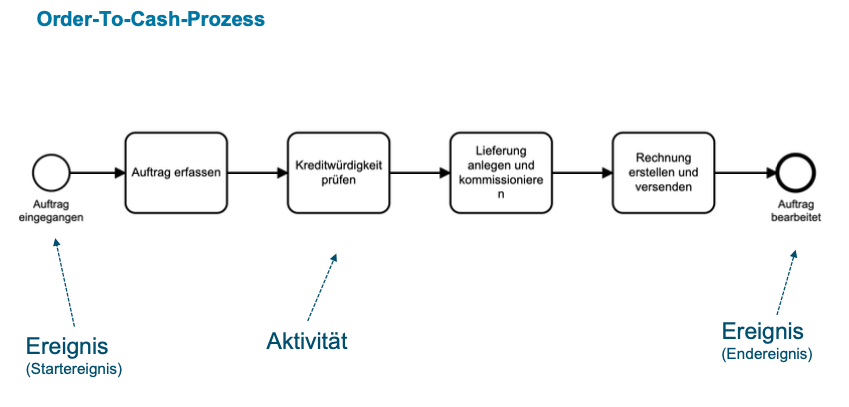
\includegraphics[width=\textwidth]{image/Elemente-Prozessmodelle.png}
        \caption{Elemente Prozessmodelle}
        \label{fig:Elemente-Prozessmodelle}
    \end{figure}
    \subsubsection*{Grundlegende Elemente}
        \begin{itemize}
            \item Aktivitäten: aus einzelschritten gebündelte Arbeitseinheit (z.B. Rechnung erstellen)
            \item Ereignis: tritt spontan auf (z.B. Kunde storniert Auftrag)
            \item Sequenzfluss: Ereignisse und Aktivitäten stehen in logischer Beziehung
            \item Startereignis: Bestimmt wann eine Prozessinstanz gestartet wird
            \item Endereignis: Bestimmt wann eine Prozessinstanz beendet, wird
        \end{itemize}
    \subsubsection*{Marken}
    Zeigen den aktuellen Schritt einer Prozessinstanz und dienen der Analyse

\subsection{Verzweigungen und Parallelisierungen}
    \subsubsection*{Exklusive ODER}
        \begin{figure}[h]
            \centering
            
\includegraphics[width=70px]{image/XOR.png}
            \caption{Exklusive ODER}
            \label{fig:XOR}
        \end{figure}
    \subsubsection*{Parallelisierung}
        \begin{figure}[h]
            \centering
            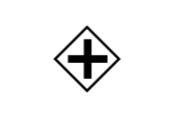
\includegraphics[width=70px]{image/Parallelisierung.png}
            \caption{Parallelisierung}
            \label{fig:Parallelisierung}
        \end{figure}
    \subsubsection*{Inklusiv Oder}
        \begin{figure}[h]
            \centering
            
\includegraphics[width=70px]{image/inklusiv-oder.png}
            \caption{Inklusiv Oder}
            \label{fig:inklusiv-oder}
        \end{figure}

\subsection{Geschäftsobjekte und Ressourcen}
    \subsubsection*{Geschäftsobjekte}
        Elemente, die innerhalb eines Prozesses verwendet oder erstellt werden. 
        \begin{itemize}
            \item Erstellen eines Angebots\textrightarrow erzeugt Angebot\textrightarrow Angebot versenden. 
            \item Symbol: Datei. Werden mit - - - -\textrightarrow Aktivitäten verbunden.
        \end{itemize}
    \subsubsection*{Ressourcen}
        Menschen, Maschinen und Materialien, die zur Durchführung von Aktivitäten benötigt werden. 
        \begin{itemize}
            \item Werden durch Bahnen dargestellt.
            \item Aktivitäten werden den Ressourcen zugeordnet.
        \end{itemize}

\subsection{Prozesszerlegung}
    \subsubsection*{Hierarchische Strukturierung}
        Zerlegung komplexer Prozesse in kleinere, handhabbare Subprozesse (Fragmente) zur besseren Übersicht und Steuerung.
    \subsubsection*{Modularisierung}
        Bildung von Modulen, die unabhängig voneinander entwickelt und gewartet werden können.

\subsection{Ereignisse und Behandlung von Ausnahmen}
    \subsubsection*{Zwischenereignisse}
        Bild (doppelter Rand)
    \subsubsection*{Ausnahmen}
        Bild (Blitz)